\tikzset{every picture/.style={line width=0.75pt}} %set default line width to 0.75pt        

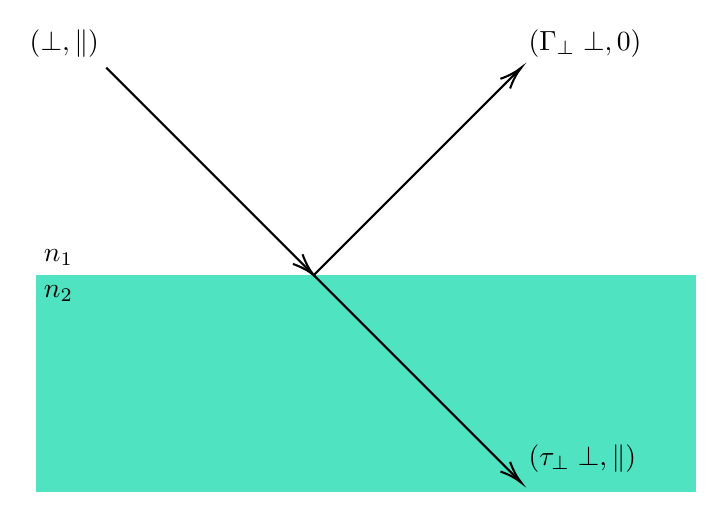
\begin{tikzpicture}[x=0.75pt,y=0.75pt,yscale=-1,xscale=1]
%uncomment if require: \path (0,504); %set diagram left start at 0, and has height of 504

%Shape: Rectangle [id:dp24828463924463207] 
\draw  [color={rgb, 255:red, 80; green, 227; blue, 194 }  ,draw opacity=1 ][fill={rgb, 255:red, 80; green, 227; blue, 194 }  ,fill opacity=1 ] (138,229) -- (455,229) -- (455,333) -- (138,333) -- cycle ;
%Straight Lines [id:da47522454577861106] 
\draw    (171.5,128.79) -- (270.09,227.38) ;
\draw [shift={(271.5,228.79)}, rotate = 225] [color={rgb, 255:red, 0; green, 0; blue, 0 }  ][line width=0.75]    (10.93,-3.29) .. controls (6.95,-1.4) and (3.31,-0.3) .. (0,0) .. controls (3.31,0.3) and (6.95,1.4) .. (10.93,3.29)   ;
%Straight Lines [id:da1053230153406346] 
\draw    (271.5,228.79) -- (370.09,327.38) ;
\draw [shift={(371.5,328.79)}, rotate = 225] [color={rgb, 255:red, 0; green, 0; blue, 0 }  ][line width=0.75]    (10.93,-3.29) .. controls (6.95,-1.4) and (3.31,-0.3) .. (0,0) .. controls (3.31,0.3) and (6.95,1.4) .. (10.93,3.29)   ;
%Straight Lines [id:da4504340662665598] 
\draw    (271.5,228.79) -- (370.09,130.2) ;
\draw [shift={(371.5,128.79)}, rotate = 135] [color={rgb, 255:red, 0; green, 0; blue, 0 }  ][line width=0.75]    (10.93,-3.29) .. controls (6.95,-1.4) and (3.31,-0.3) .. (0,0) .. controls (3.31,0.3) and (6.95,1.4) .. (10.93,3.29)   ;

% Text Node
\draw (140,225.6) node [anchor=south west] [inner sep=0.75pt]    {$n_{1}$};
% Text Node
\draw (140,232.4) node [anchor=north west][inner sep=0.75pt]    {$n_{2}$};
% Text Node
\draw (169.5,125.39) node [anchor=south east] [inner sep=0.75pt]    {$( \perp ,\parallel )$};
% Text Node
\draw (373.5,125.39) node [anchor=south west] [inner sep=0.75pt]    {$( \Gamma_{\perp}\perp,0)$};
% Text Node
\draw (373.5,325.39) node [anchor=south west] [inner sep=0.75pt]    {$( \tau_{\perp}\perp , \parallel )$};


\end{tikzpicture}
